\documentclass{article}
\usepackage[english]{babel}
\usepackage[utf8]{inputenc}
\usepackage{amsmath}
\usepackage{graphicx}
\usepackage[colorinlistoftodos]{todonotes}
\usepackage{graphics}

\title{CIS 542 Lab 1}

\author{Gabrielle Merritt}

\date{\today}
\begin{document}
\maketitle
\section{Installing virtual box} 
Installing virtual box was quite easy and painless, I was able to complete this process in about 10 to 15 minutes. I've used parallels before and all my computers are dual booted with Ubuntu so I'm fairly familiar with the process. Though it was very nice that since it's a virtual machine I didn't have to worry about properly partitioning my hard drive. 

\section{SSH into virtual box} 
I had some difficulty actually accessing my virtual box from OSX. 
The default network setting (NAT) could not ping itself, and had very slow ping times to other website (ie. google.com) 
\paragraph{}
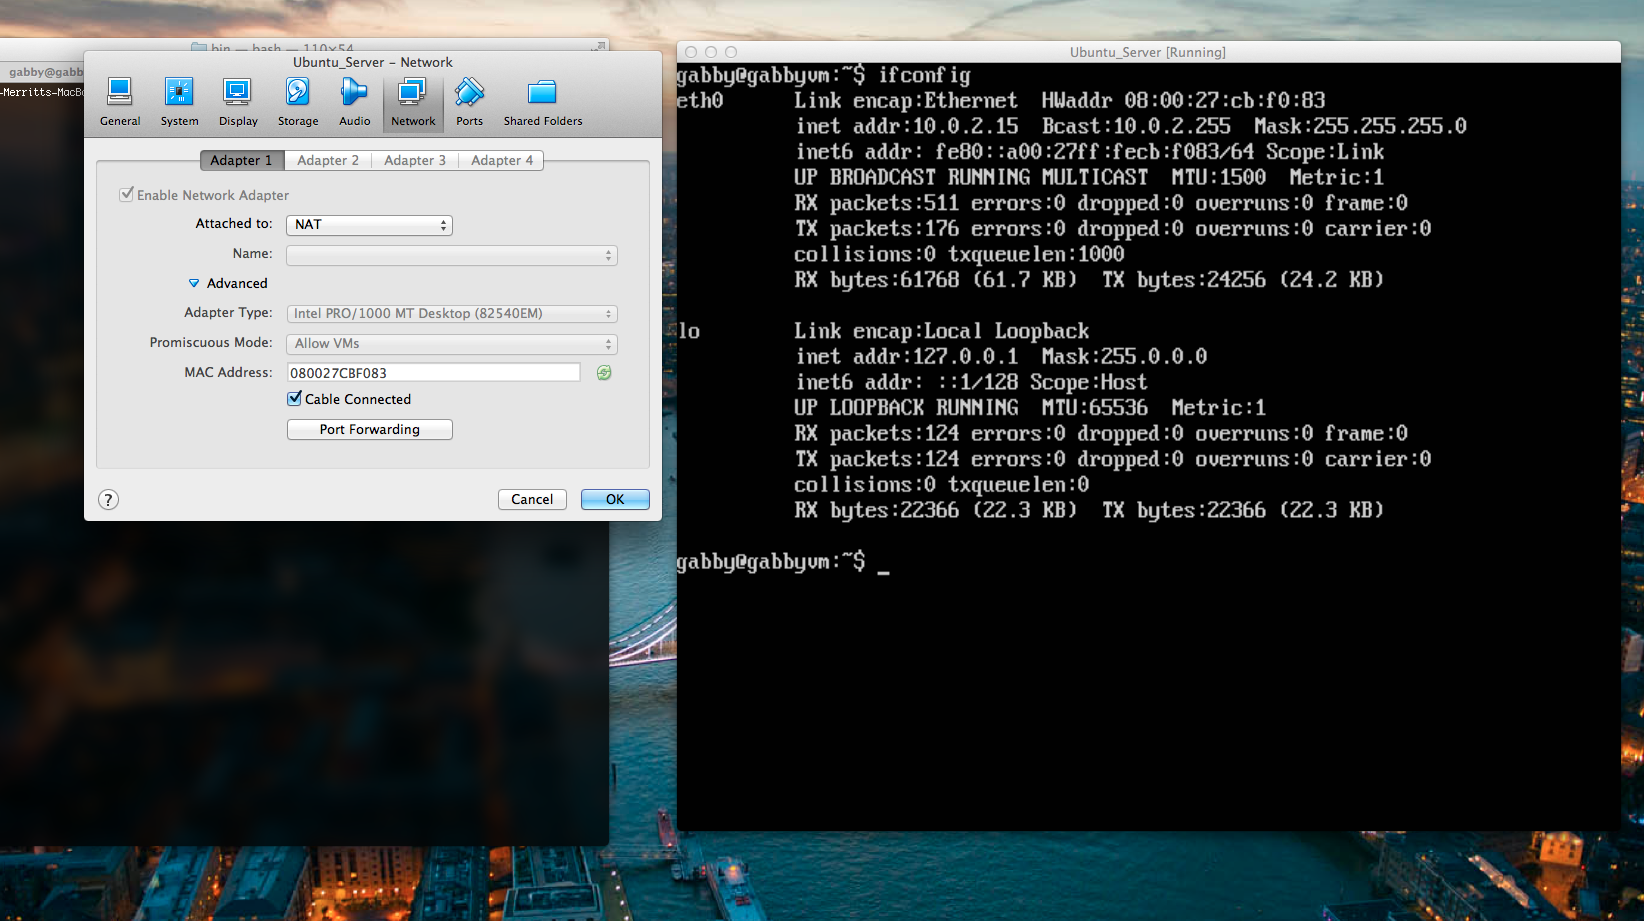
\includegraphics[width =\linewidth]{NAT.png}
\paragraph{}
I noticed the bridged mode network connection for Virtual box assigned the vm an interface to connect to that was bridged to my mac's wifi, so I selected that mode, and restarted the network interface, then requested a new ip address.
\paragraph{}
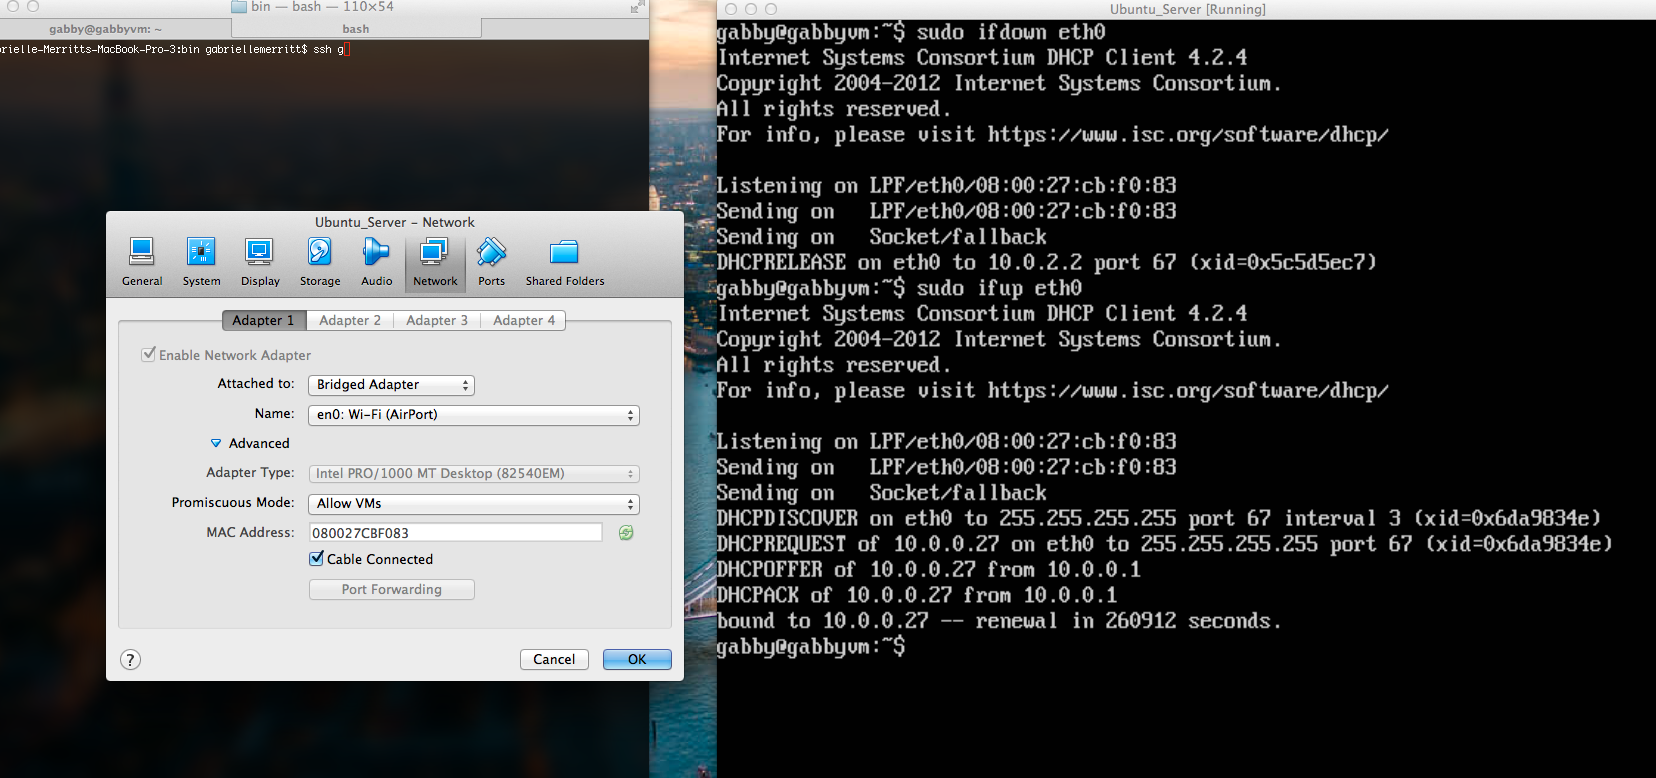
\includegraphics[width = \linewidth]{Bridge.png}

\section{Setting up SSH keys}
I was able to set up ssh key by transferring my ssh pub key to the authorized keys file on my virtual machine. However I could only do this from my linux machine because I can't install open ssh or the copy-ssh-id on to OSX

\end{document}
